\documentclass[a4paper, 12pt]{article} %tipo de documento e opções gerais
\usepackage[utf8]{inputenc} %codificação
\usepackage[T1]{fontenc} %codificação
\usepackage[portuguese]{babel}  %idioma
\usepackage{amsmath,amssymb,amsfonts,amsthm} %padrões em formato matemático
\usepackage[a4paper,top=3cm,bottom=2cm,left=3cm, right=2cm]{geometry} %margens
\usepackage{indentfirst} %primeiro parágrafo com margem
\usepackage{float} %fixar imagens e tabelas
\usepackage{multicol} %várias colunas
\usepackage{multirow} %várias linhas
\usepackage{graphicx} %colocar imagens 
\usepackage{anyfontsize} %qualquer tamanho de letra
\usepackage{setspace} %espaçamento
\usepackage[titles]{tocloft} %padrões de sumário
\usepackage{fontspec} %outros tipos de fonte
\usepackage{fancyhdr} %padronizar o formato do Header
\usepackage[resetlabels,labeled]{multibib} %bibliografia
\usepackage{newfloat} %alterar nome do quadro
\usepackage{tabls} %pacote para espaçamento de linhas
%\usepackage{titlesec}
\usepackage{makecell}
\usepackage{shadowtext}
\usepackage{eso-pic,graphicx}
\usepackage{tikz} %trabalhar com imagens e add background
\usepackage[absolute,overlay]{textpos}
\usepackage{calc} %para funçoes como \widthof
\usepackage{hyperref}
\usepackage{afterpage} % contracapa

\newcommand\blankpage{% código para a contracapa
    \null
    \thispagestyle{empty}%
    \addtocounter{page}{-1}%
    \newpage}

%definindo novo estilo de pagina
\makeatletter
\def\ps@Padrao{
    %número da página com cor clara e no canto
    \def\@oddfoot{\textcolor{white}{\null\hfill\thepage}}%
    \def\@evenfoot{\thepage}%
    %definindo cabeçado para o canto
    \def\@evenhead{\null\hfil\slshape\leftmark }%
    \def\@oddhead{{\slshape\rightmark\hfill \includegraphics[scale=0.2]{estat.png}}}} %cabeçalho
\makeatother

\pagestyle{Padrao}

\setmainfont{Arial} %fonte arial
\setstretch{1.5} %espaçamento
\setlength\tablinesep{5pt} %espaço entre as células da tabela

% ALTERANDO O TÍTULO DAS TABELAS E FIGURAS
\addto\captionsenglish{%
  \renewcommand\tablename{Tabela}
  \renewcommand\figurename{Figura}
}
\DeclareFloatingEnvironment[listname=loq, listname={Lista de Quadros}]{quadro}

% ALTERANDO O SUMÁRIO
\makeatletter
\renewcommand\tableofcontents{
  \null\hfill\textbf{\Large\contentsname}\hfill\null\par
  \@mkboth{\MakeUppercase\contentsname}{\MakeUppercase\contentsname}%
  \@starttoc{toc}}
\makeatother	
\addto\captionsenglish{
  \renewcommand{\contentsname}{Sumário}
  }

\clearpage

\begin{document}
\begin{titlepage}

\center
\tikz[remember picture,overlay] \node[opacity=1,inner sep=0pt] at (current page.center){\includegraphics[width=\paperwidth,height=\paperheight]{capa.png}};

\begin{minipage}{16cm}
\begin{flushright}
% posições do título (substituir o segundo parâmetro do begin{textblock}
% 1 linha:  (4cm, 8.38cm)   nao esquecer de cuidar
% 2 linhas: (4cm, 7.75cm)   do tamanho das fontes
% 3 linhas: (4cm, 7.15cm)   e o espaçamento delas
% 4 linhas: (4cm, 6.55cm)
% 5+ linhas: diminuir tamanho da fonte pra caber em 4

\begin{textblock*}{16cm}(4cm, 7.75cm) %reposicione aqui

    %\fontsize{tamanho}{espaçamento de linha}
    {\fontsize{38}{22}\selectfont Estudo Descritivo da \\ Indústria Cinematográfica \par}
    %aplique \\ para saltar linhas pra rearranjar as palavras do título e ficarem melhor distribuídas
    
    %\par é para delimitar o parágrafo e poder aplicar efeitos de espaçamento entre linhas
\end{textblock*}
\end{flushright}
\end{minipage}

\vspace*{10cm}
    %{\fontsize{38}{150}\selectfont Análise do consumo médio    anual de obras de pavimentação no Distrito\par}

\begin{flushright}
\begin{minipage}{6cm} 
 \parbox[t]{8cm}{\textbf{Consultores Responsáveis:}\\ 
Davi Dantas Erthal \\
} \\ \\
\parbox[t]{5cm}{\textbf{Requerente:}\\ 
Floriano Peixoto\\
}
\end{minipage}
\end{flushright}
\vspace{2cm}

\includegraphics[scale=0.48]{estat.png}

\vfill
\end{titlepage}

\tableofcontents
\thispagestyle{empty}
\newpage

%========================INTRODUÇÃO=======================






\section{Introdução}
\AddToShipoutPictureBG{\includegraphics[width=\paperwidth,height=\paperheight]{pagina-comum.png}}

O seguinte projeto tem como propósito analisar o as características dos filmes lançados ao longo dos anos a fim de sanar as questões exigidas pelo cliente. Será feita uma análise exploratória dos dados, buscando compreender suas informações.



Para tal, serão realizadas análises descritivas individuais das variáveis, além de pesquisas sobre as correlações entre as mesmas. O banco de dados foi fornecido pelo cliente e foi construído com base em dados do IMDb e de dados retirados de plataformas de streaming. Para realização foi utilizado o software rStudio em sua versão mais atual 4.0.0.

%========================METODOLOGIA============================
\newpage
\section{Metodologia}



Para o estudo deste documento foram utilizadas medidas descritivas como média, mediana, desvio-padrão e quartis. Além disso foram usados gráficos de linhas, dispersão, colunas, boxplots, além de tabelas e quadros de medidas.

A média é a soma dos valores observados divididos pelo número de observações. A mediana é o valor observado que mais se aproxima da média. O desvio-padrão está relacionado a como os dados estão distribuídos, quanto mais alto mais os valores tendem a se desviar da média. O primeiro quartil (1° Quartil ou $Q_1$ ou Quartil Inferior) indica o valor posicionado ao 1/4 dos dados ordenados. O terceiro quartil (3° Quartil ou $Q_3$ ou Quartil Superior) indica o valor posicionado aos 3/4 dos dados ordenados.

As Figura 2 e 3 se referem a gráficos de dispersão que são utilizados para perceber o comportamento de uma variável em relação à outra, onde cada ponto representa uma observação. Já as figuras 8 e 9 correspondem a boxplots, neles pode-se ter uma maior noção de como certos dados estão distribuídos, pois contém informações como, média, mediana, amplitude e quartis. Os valores que aparecem como pontos isolados no boxplot são denotados como "outliers".

%=================================ANÁLISES=====================


\newpage
\section{Análises}

%AS ANÁLISES SERÃO FEITAS SEGUINDO AS QUESTÕES REQUERIDAS PELO CLIENTE:
% 1 - Análise da Quantidade de Lançamentos por Ano
% 2 - Análise da Relação entre a Duração dos Filmes e seu Ano de Lançamento
% 3 - Análise da Influência da Duração do Filme na Nota do Rotten Tomatoes
% 4 - Análise da Distribuição da Classificação Indicativa do Filme por Plataforma
% 5 - Análise do IMDb das plataformas Netflix e Prime Video
% 6 - Top 5 Diretores Segundo a Nota do IMDb

%======================QUESTÃO 1=====================================

\subsection{Análise da Quantidade de Lançamentos por Ano}

Esta seção tem como objetivo analisar o número de filmes lançados em cada ano. Para essa análise foi utilizado o seguinte gráfico de linha.

\begin{figure}[H]
\cantering
\caption{Gráfico de linha da variável Quantidade de Lançamentos}
\label{graf_lancamentos_ano}
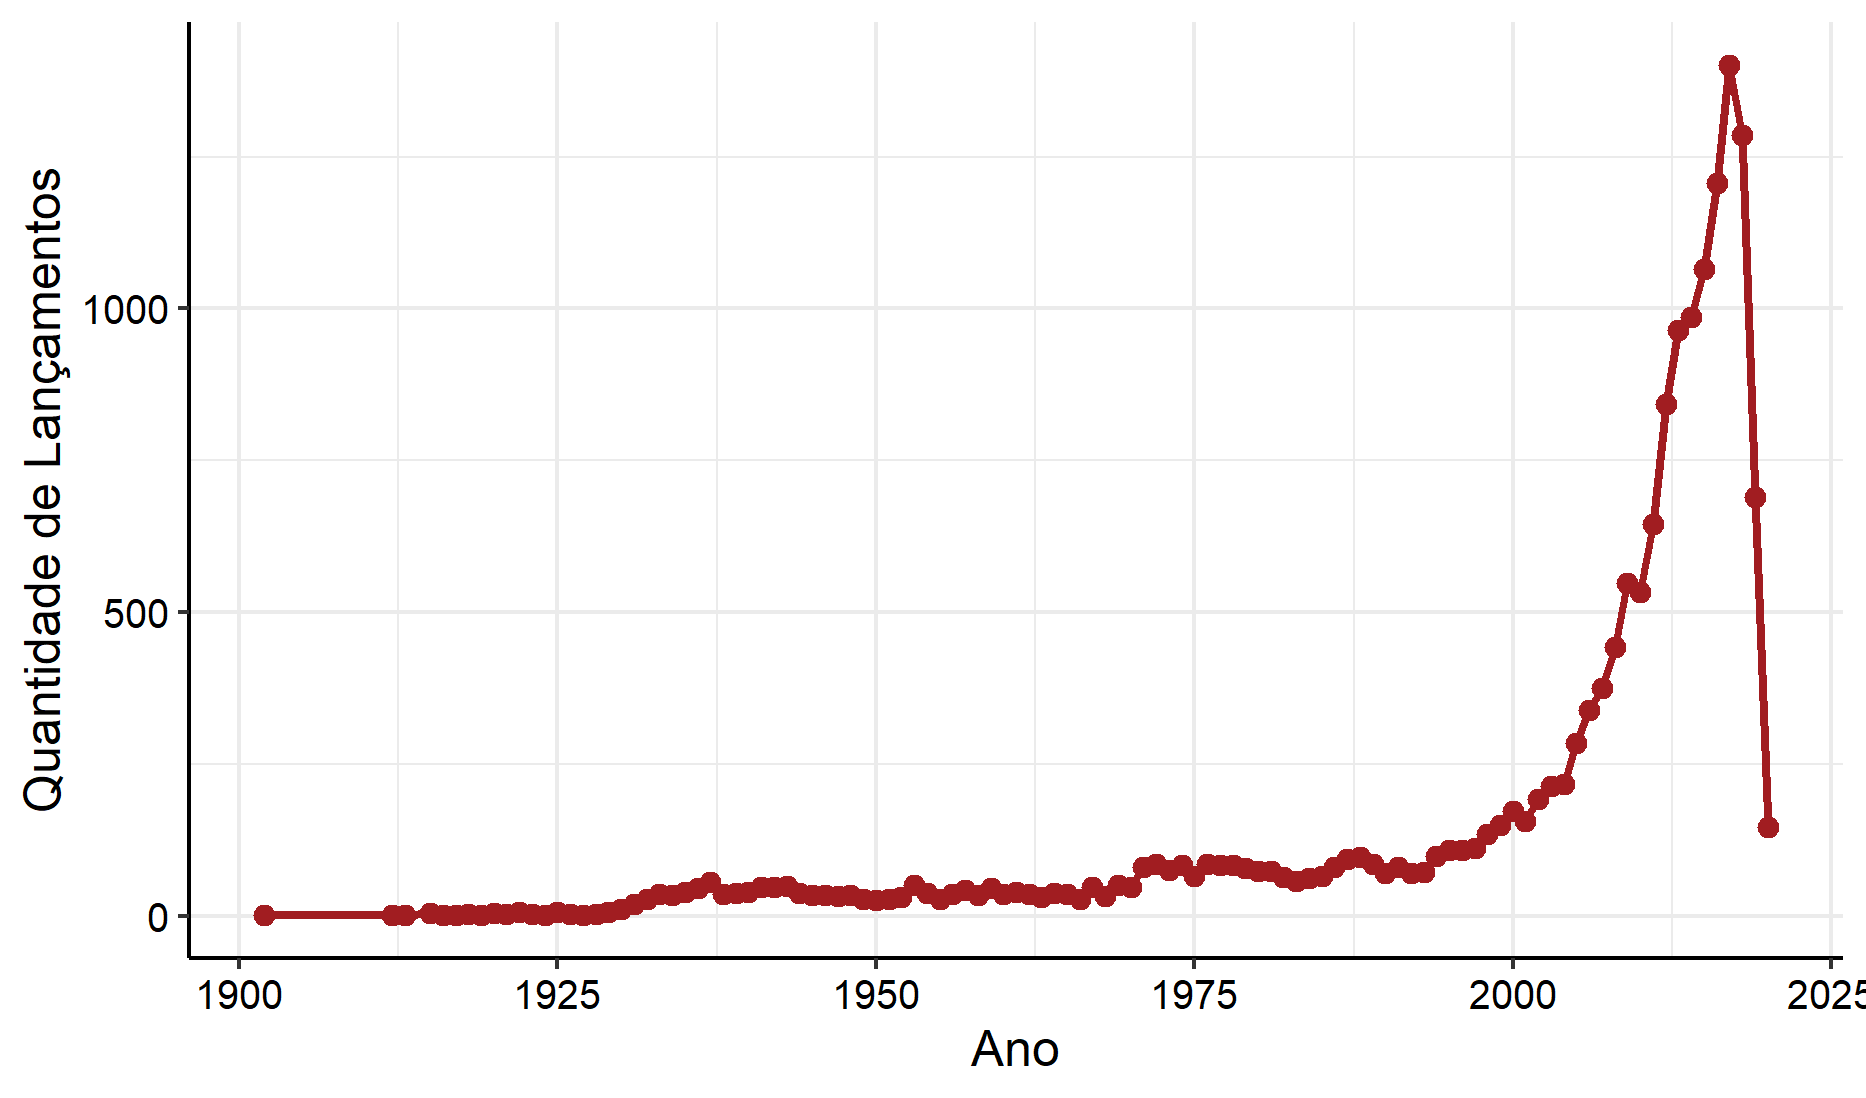
\includegraphics[scale=1]{graf_lancamentos_ano.png}
\end{figure}




Com a análise da Figura \ref{graf_lancamentos_ano}, nota-se que houve um crescimento considerável no número de lançamentos de filme no começo do século XXI, e que no último ano (2020) aconteceu uma queda grave nesse número. %Vale ressaltar que um visível fator para tal queda foi a pandemia global do vírus COVID-19 que afetou todas as áreas da economia, inclusive a da produção de filmes.

%======================QUESTÃO 2=====================================

\subsection{Análise da Relação entre a Duração dos Filmes e seu Ano de Lançamento}

Esta seção tem como propósito indicar se há ou não correlação entre a duração dos filmes e seu ano de lançamento. Para tal foi utilizado o seguinte gráfico de dispersão.

\begin{figure}[H]
\cantering
\caption{Gráfico de dispersão das variáveis Duração do Filme e Ano de Lançamento}
\label{box_uni1}
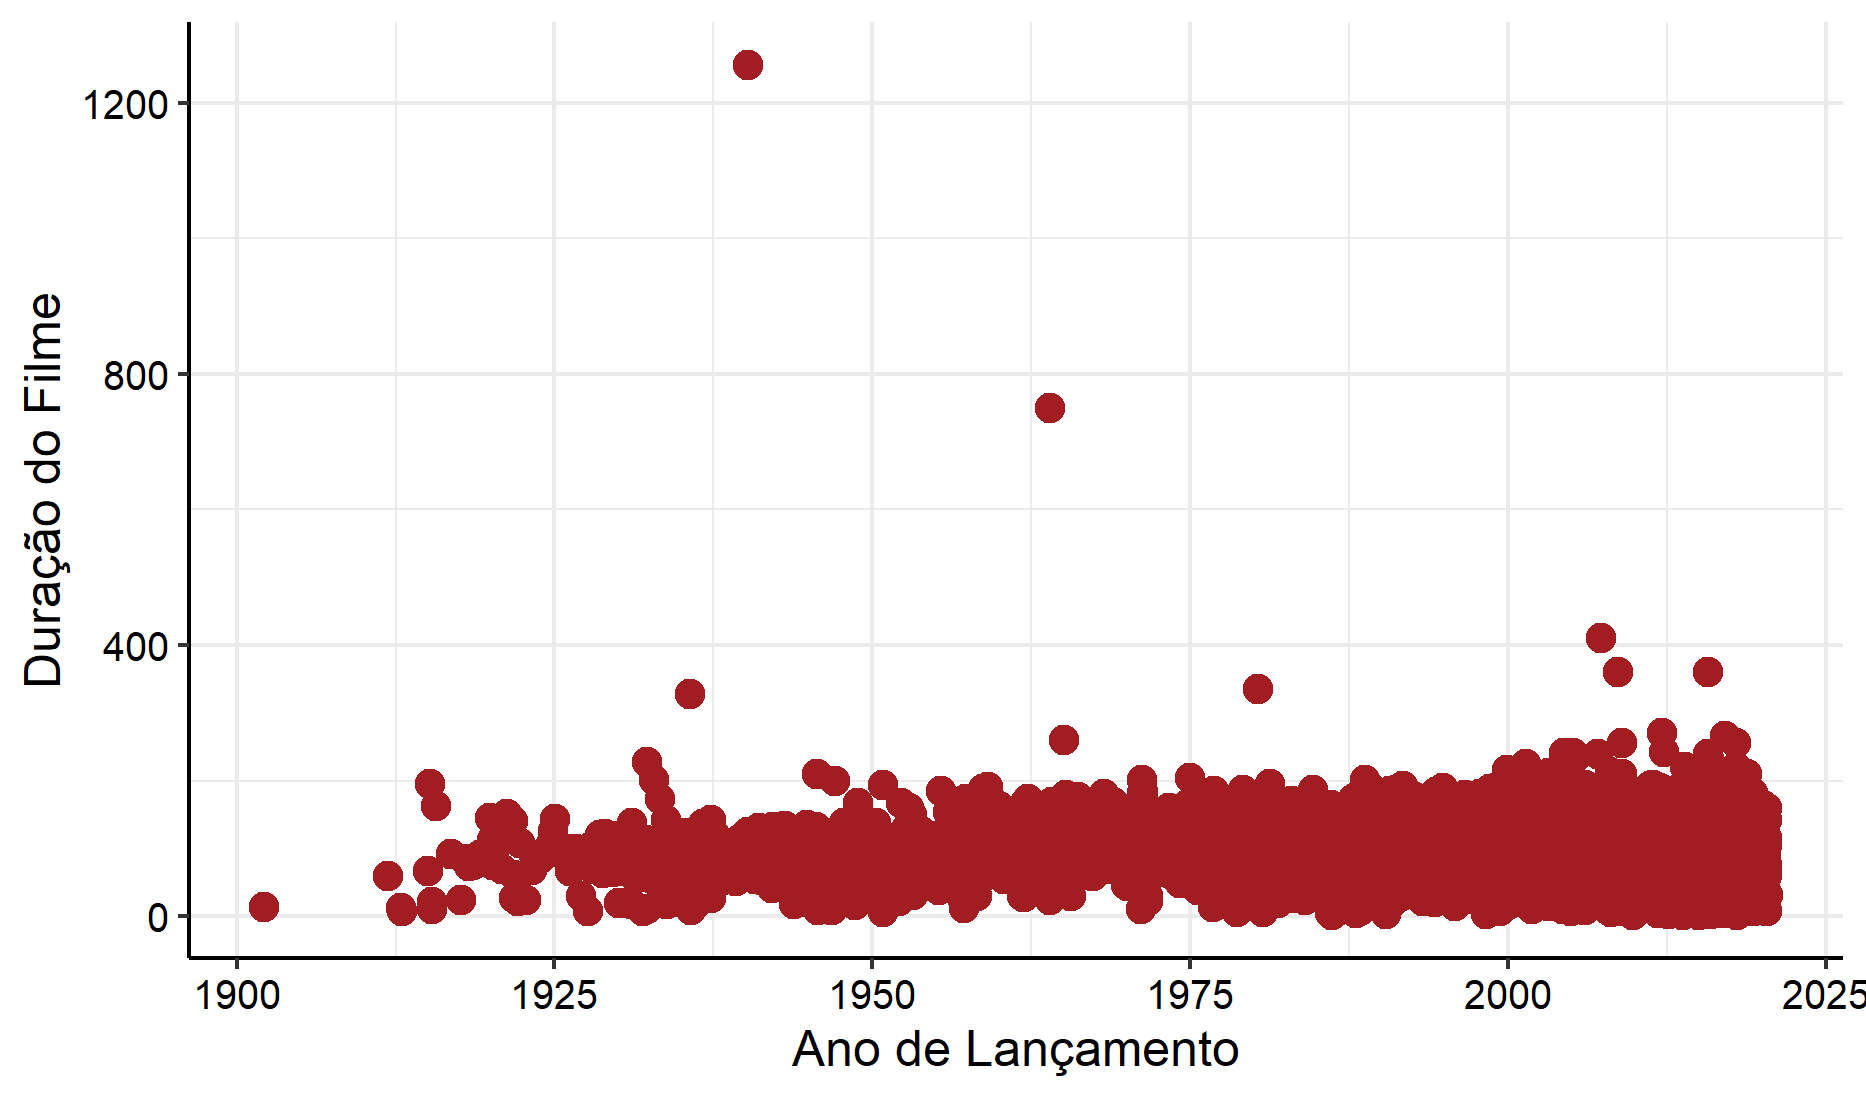
\includegraphics[scale=1]{graf_duracao_ano.png}
\end{figure}





Pela análise da Figura \ref{box_uni1}, percebe-se que provavelmente não há correlação entre as duas variáveis dado que independente do ano de lançamento as durações seguem um mesmo padrão.

%======================QUESTÃO 3=====================================

\subsection{Análise da Influência da Duração do Filme na Nota do Rotten Tomatoes}

Esta seção tem como finalidade estudar se há influência da duração do filme na nota do Rotten Tomatoes com auxílio do seguinte gráfico de dispersão.

\begin{figure}[H]
\cantering
\caption{Gráfico de dispersão das variáveis Duração do Filme e Nota do Filme no Rotten Tomatoes}
\label{box_uni2}
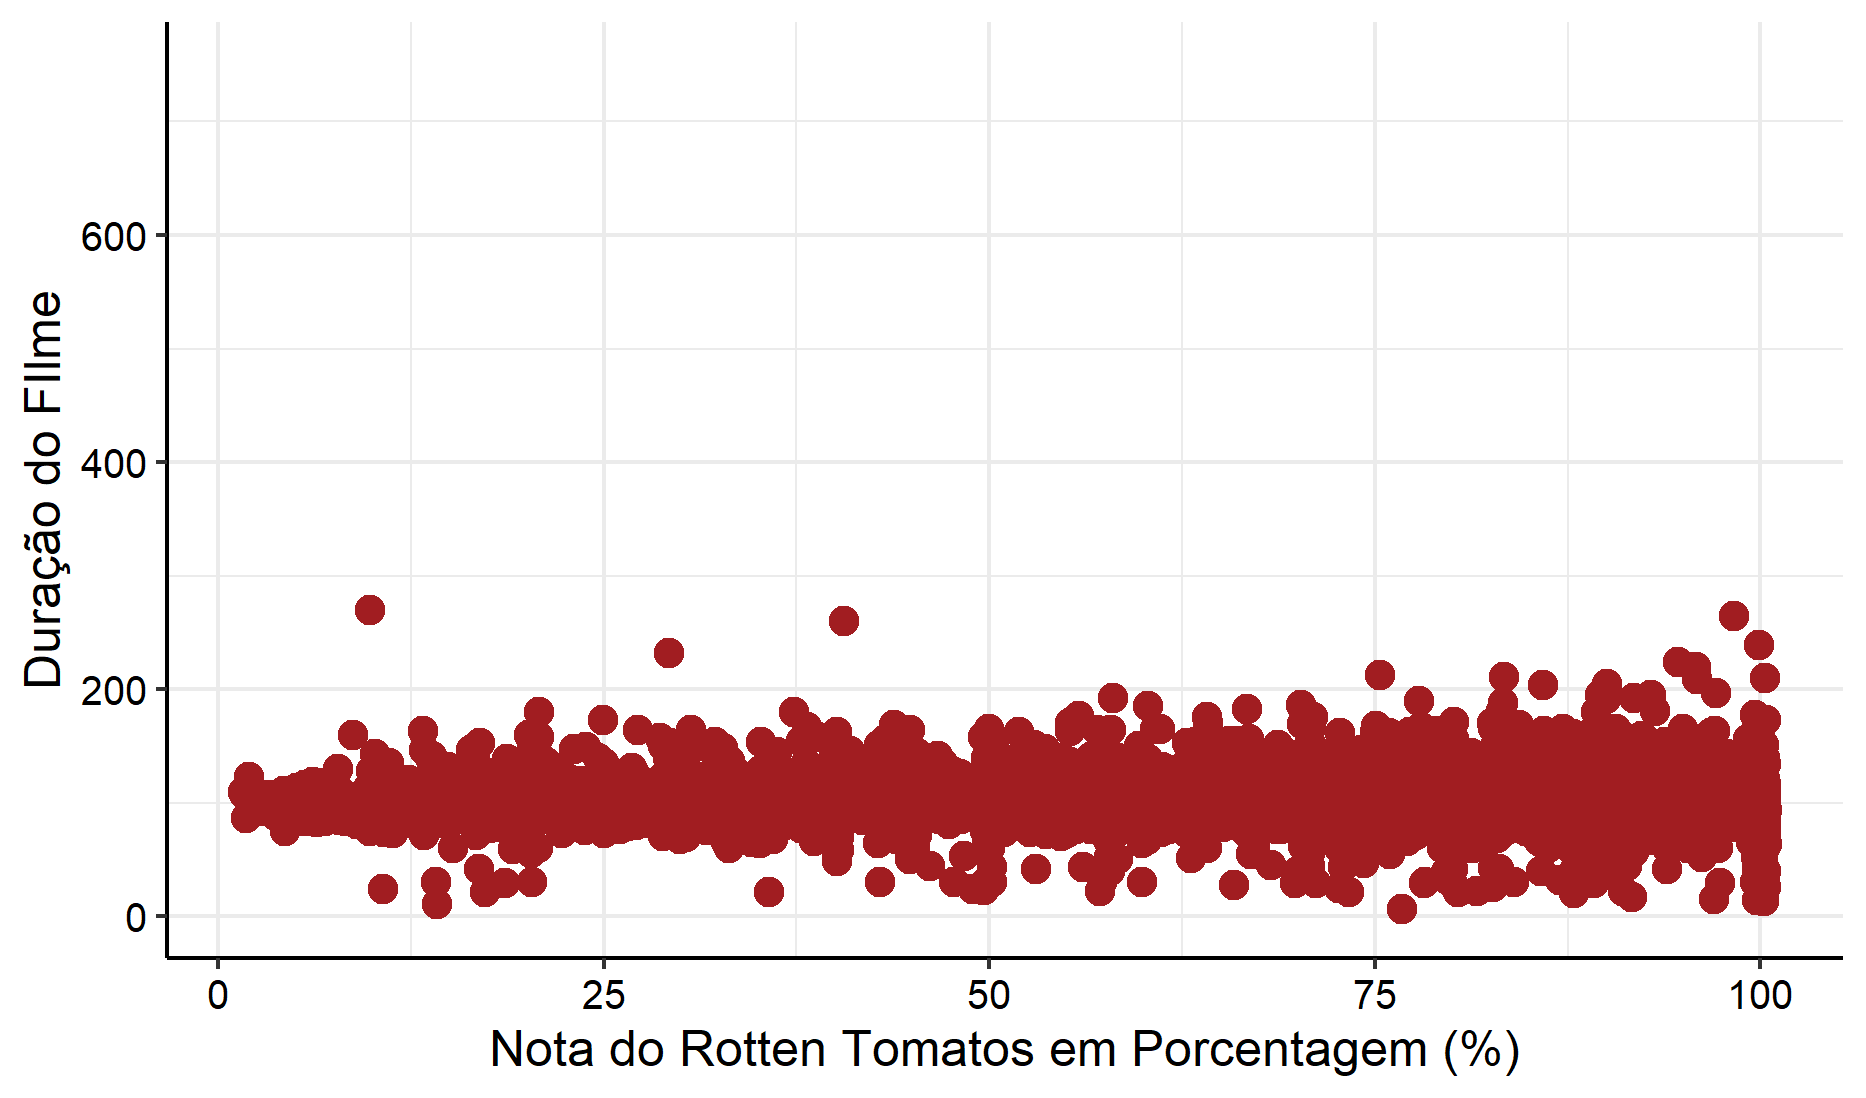
\includegraphics[scale=1]{graf_duracao_rotten.png}
\end{figure}

Analisando a Figura \ref{box_uni2} nota-se que provavelmente não há correlação entre a duração do filme e a nota do site Rotten Tomatoes devido as durações estarem bem distribuídas pelas notas. 



%======================QUESTÃO 4=====================================

\subsection{Análise da Distribuição da Classificação Indicativa do Filme por Plataforma}

Esta seção tem como intuito analisar a classificação indicativa do filme por plataforma. Para isso foram utilizados os seguintes gráficos e uma tabela.

%========================GRÁFICOS CLASSIFICAÇÃO INDICATIVA======





%===================Gráfico Netflix
\begin{figure}[H]
\cantering
\caption{Gráfico de colunas da distribuição da classificação indicativa na plataforma Netflix}
\label{box_uni3}
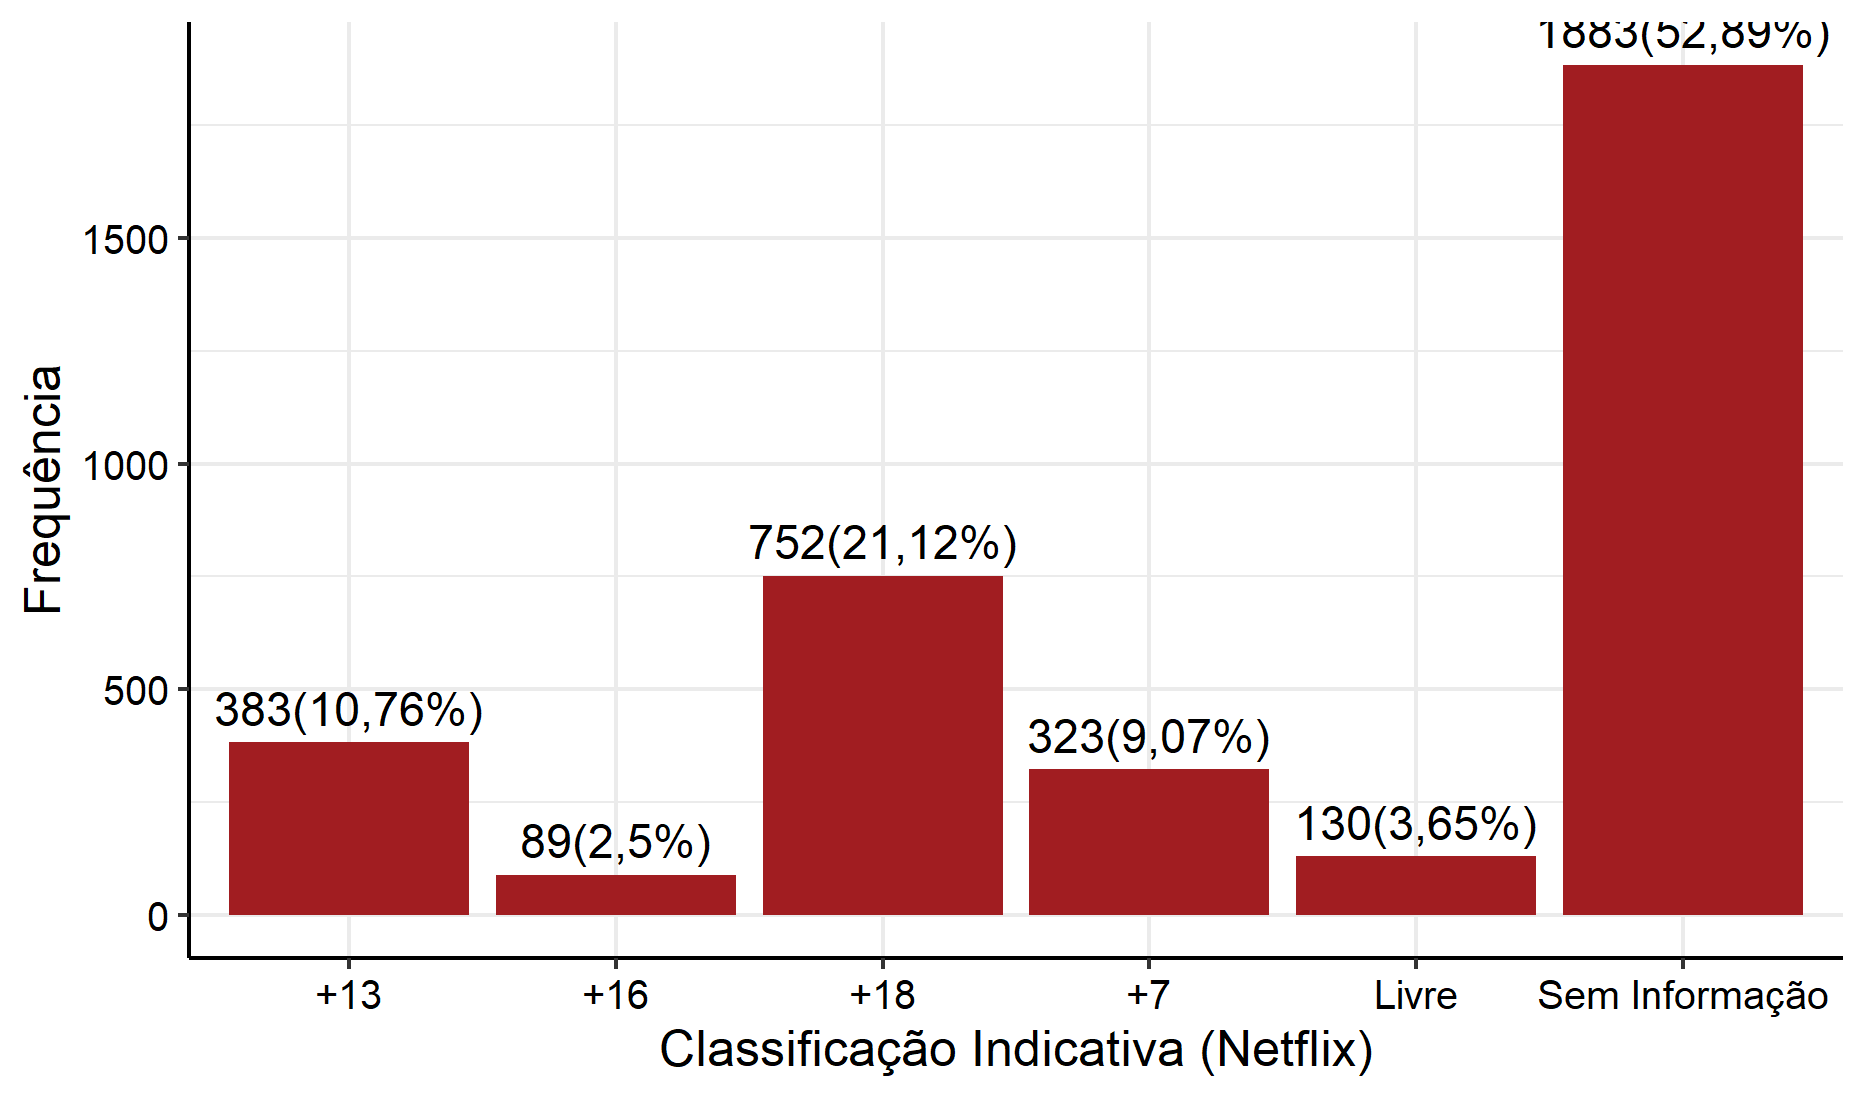
\includegraphics[scale=1]{CORREC_NETFLIX.png}
\end{figure}

%=================Gráfico Hulu
\begin{figure}[H]
\cantering
\caption{Gráfico de colunas da distribuição da classificação indicativa na plataforma Hulu}
\label{box_uni4}
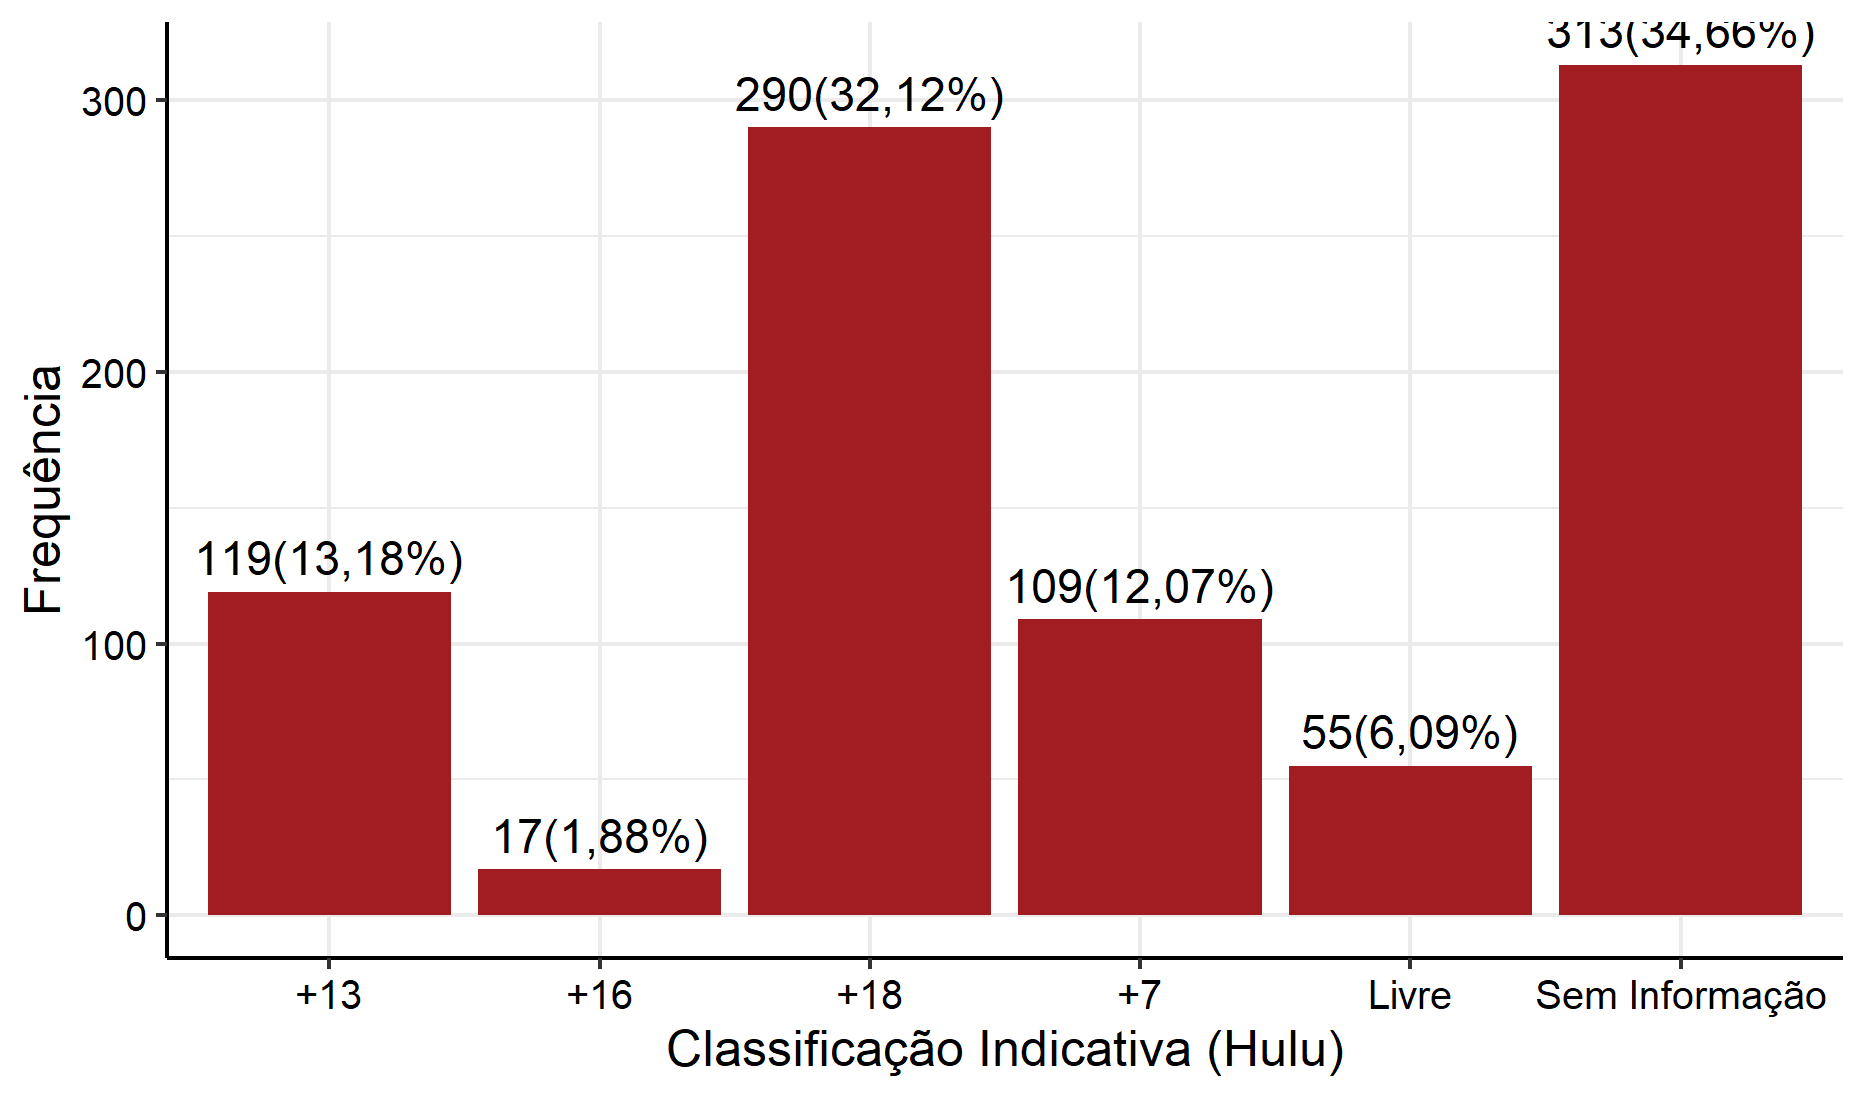
\includegraphics[scale=1]{CORREC_HULU.png}
\end{figure}

%===================Gráfico Prime Video
\begin{figure}[H]
\cantering
\caption{Gráfico de colunas da distribuição da classificação indicativa na plataforma Prime Video}
\label{box_uni5}
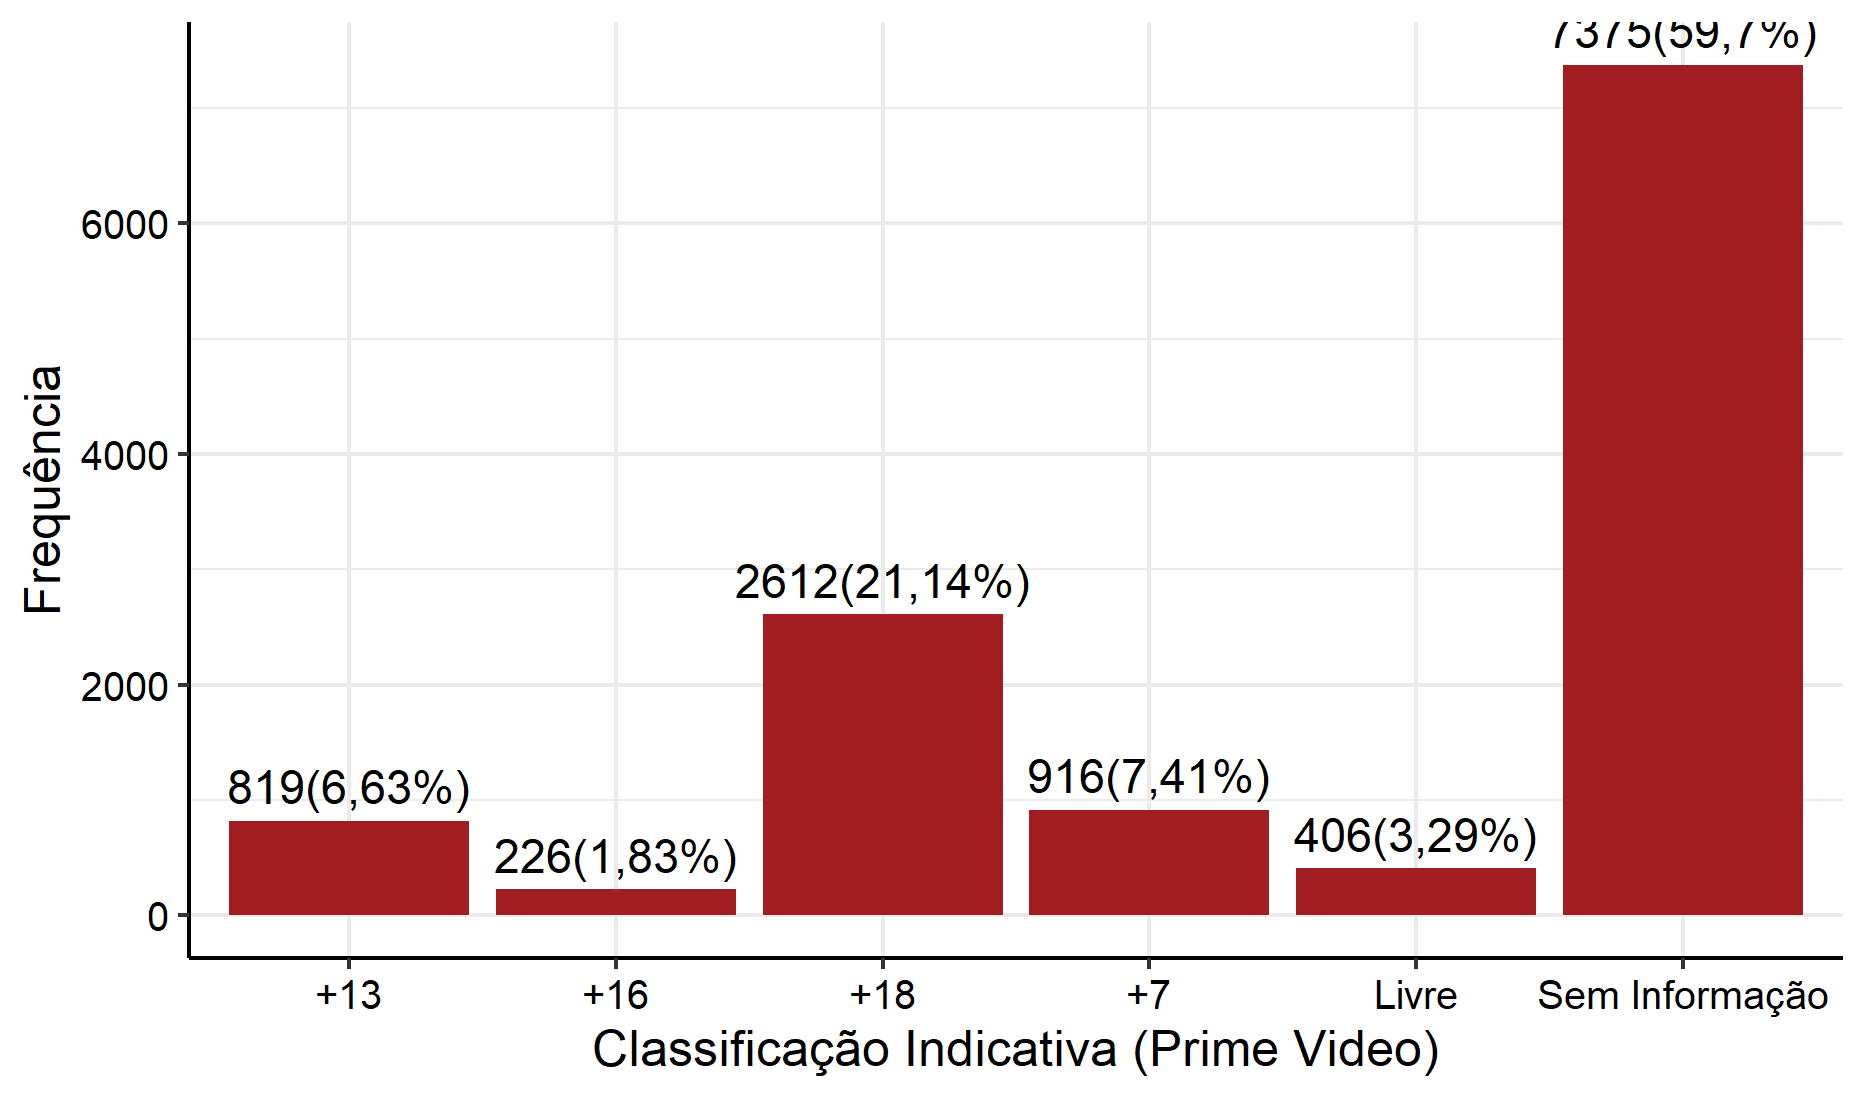
\includegraphics[scale=1]{CORREC_PRIMEVIDEO.png}
\end{figure}

%======================Gráfico Disney
\begin{figure}[H]
\cantering
\caption{Gráfico de colunas da distribuição da classificação indicativa na plataforma Disney}
\label{box_uni6}
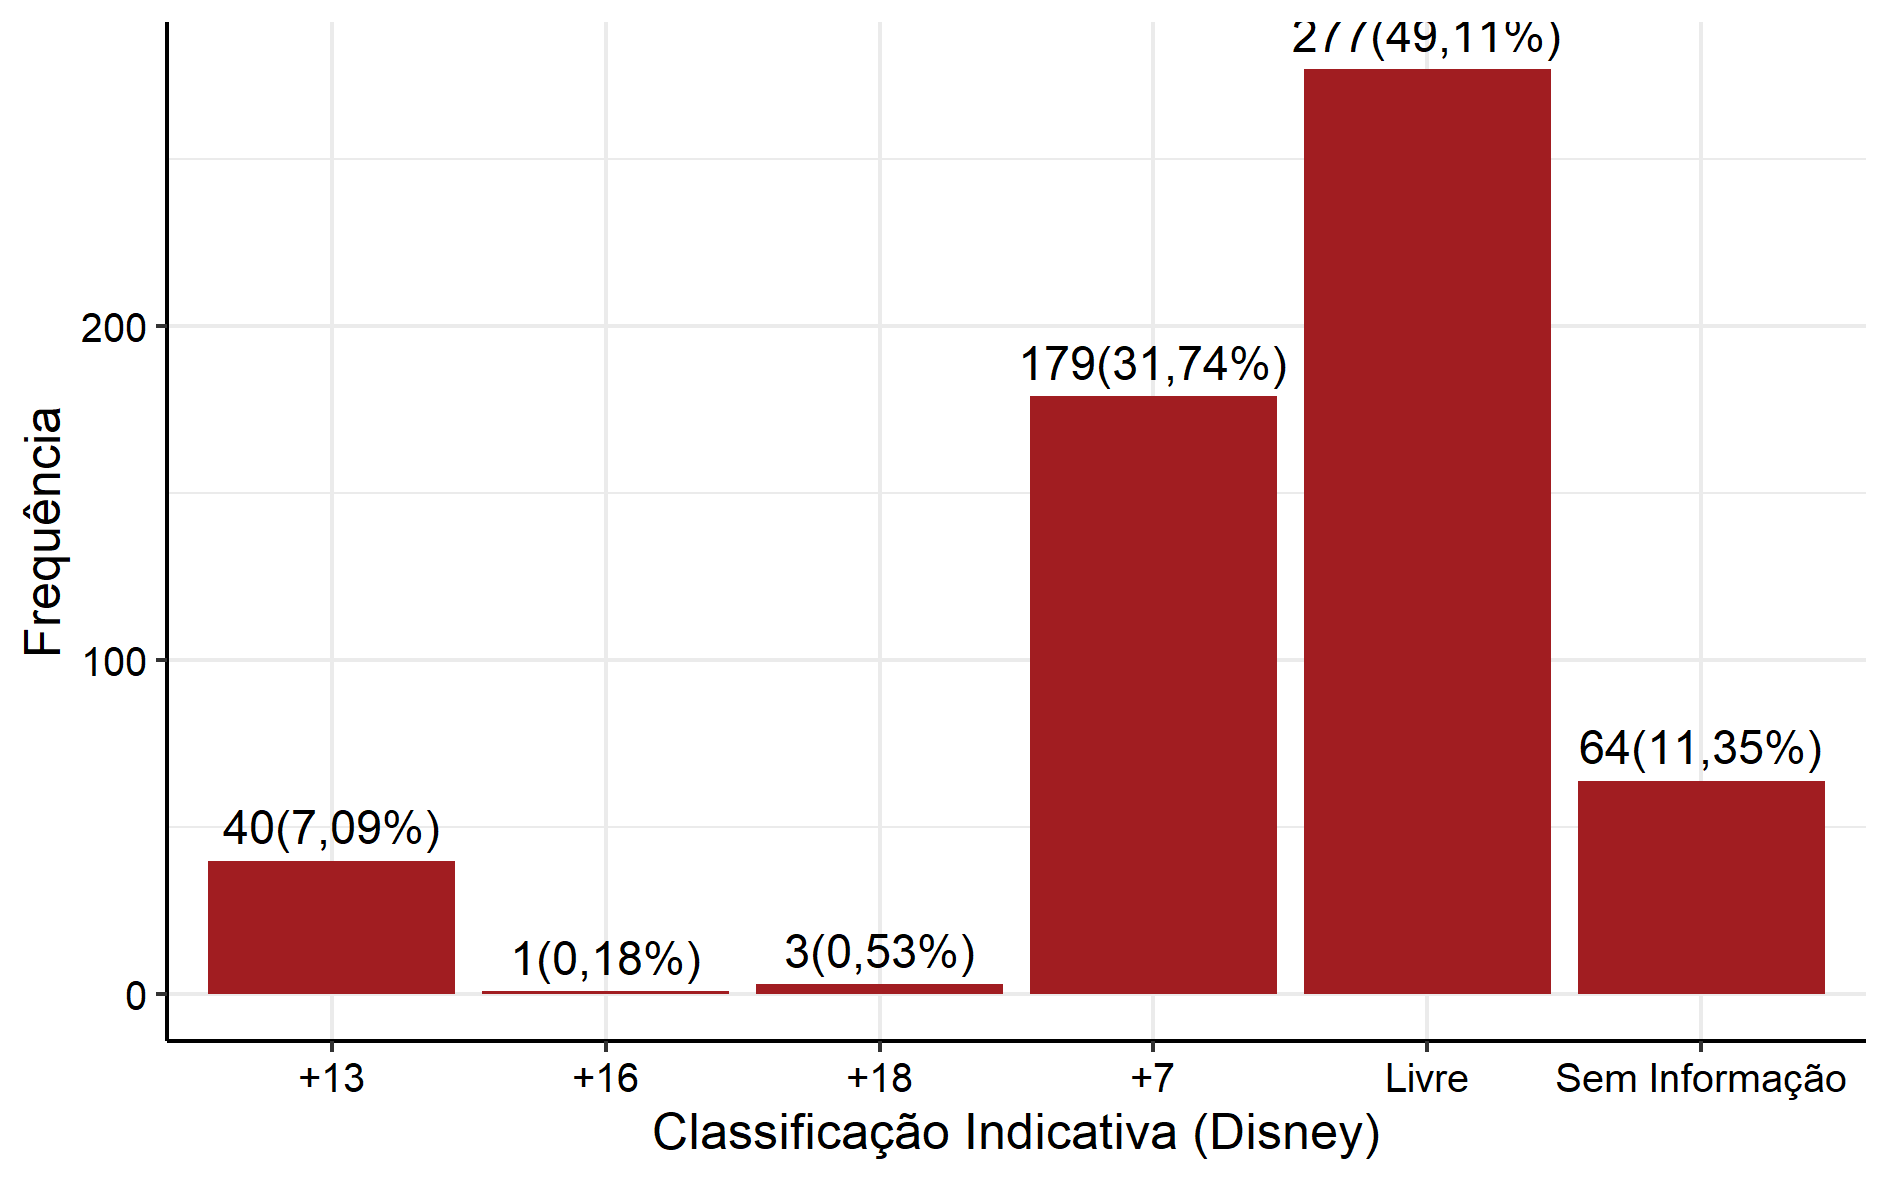
\includegraphics[scale=1]{CORREC_DISNEY2.png}
\end{figure}

%===========TABELAS CLASSIFICAÇÃO INDICATIVA===================




Pelas análises das Figuras \ref{box_uni3}, \ref{box_uni4}, \ref{box_uni5} e \ref{box_uni6} nota-se que a plataforma Disney tem uma tendência à filmes com classificação menor (+7 = 31,74\% e Livre = 49,11\%) e tem poucos filmes com classificação 18+ (0,53\%) em seu catálogo.

Enquanto as demais plataformas se assemelham a respeito da distribuição de classificação indicativa.

%======================QUESTÃO 5=====================================



\subsection{Análise do IMDb das plataformas Netflix e Prime Video}

Esta seção tem como objetivo comparar as notas no IMDb das plataformas Netflix e Prime Video. Para isso foram utilizados dois bloxplots, um para cada plataforma e um quadro de medidas.

\begin{figure}[H]
\cantering
\caption{Boxplot das notas no IMDb da plataforma Netflix}
\label{box_uni}
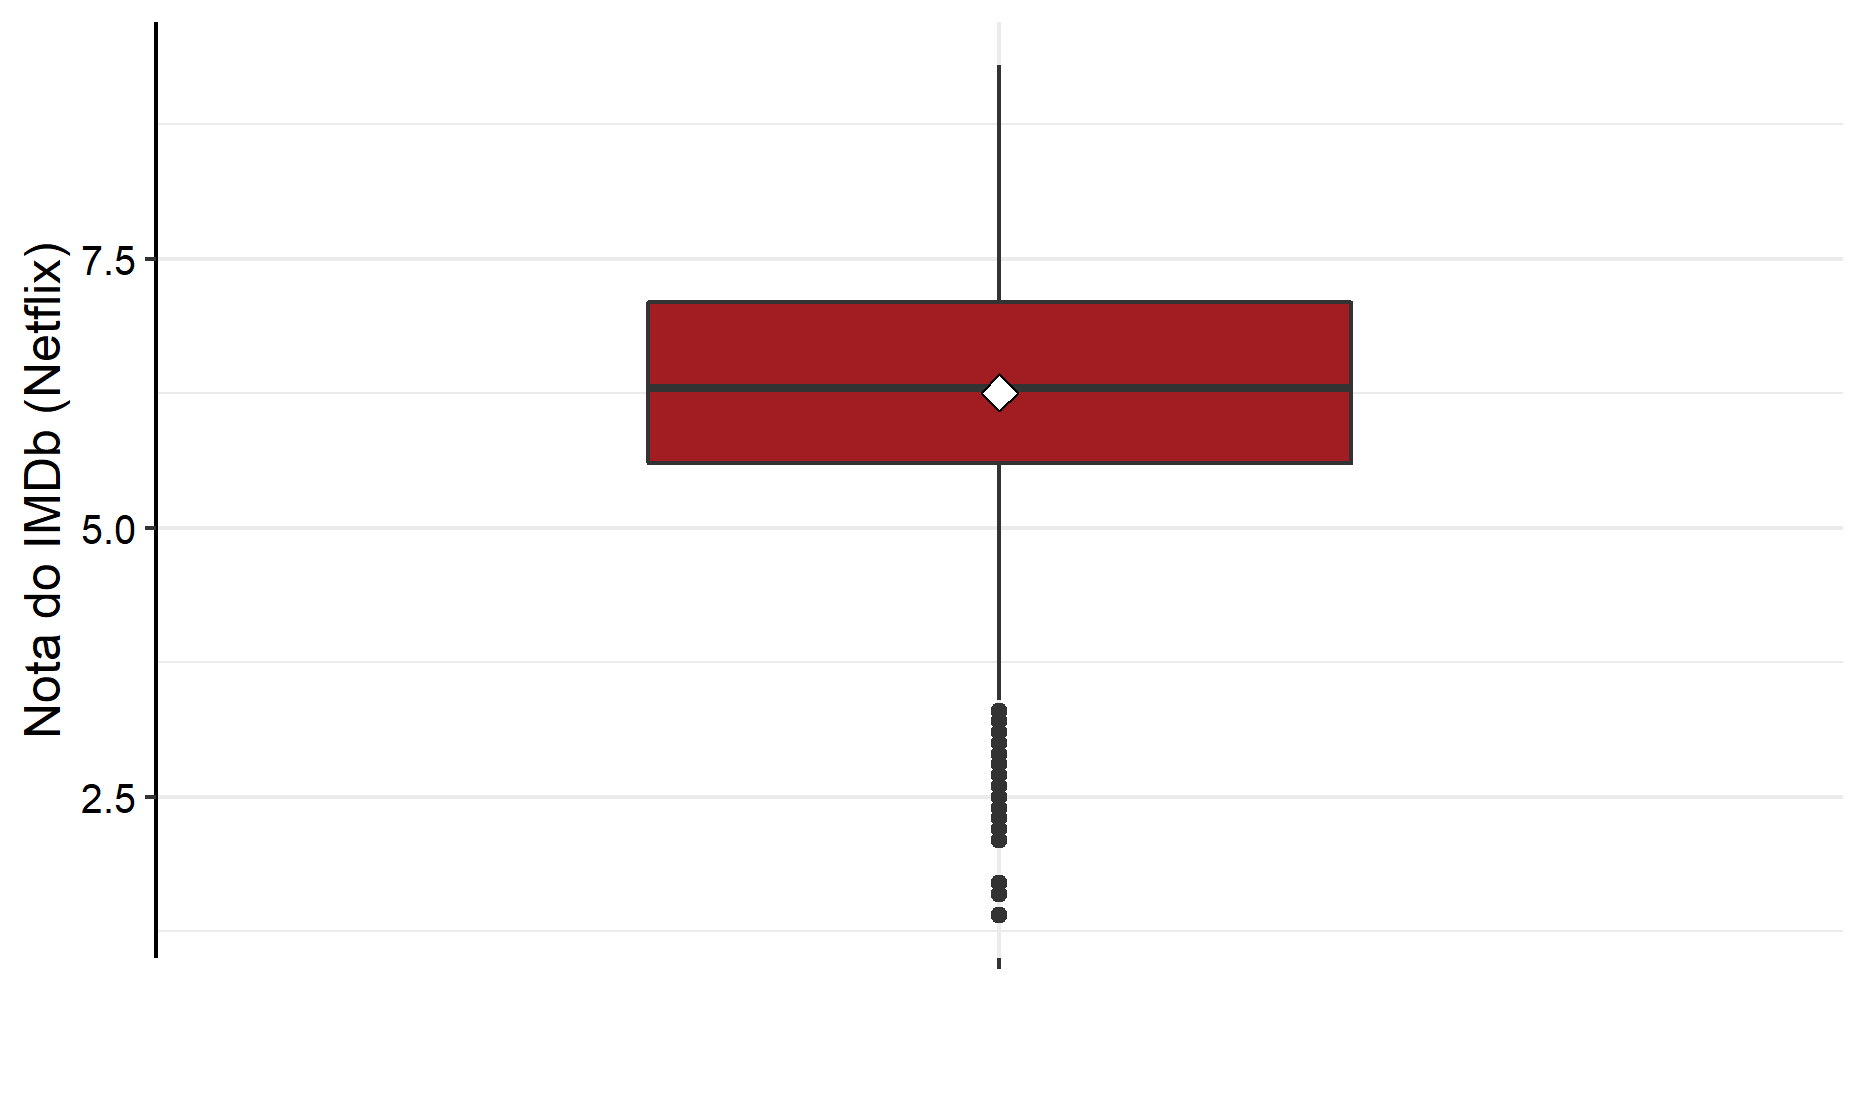
\includegraphics[scale=1]{graf_netflix_imdb.png}
\end{figure}

\begin{figure}[H]
\cantering
\caption{Boxplot das notas no IMDb da plataforma Prime Video}
\label{box_uni}
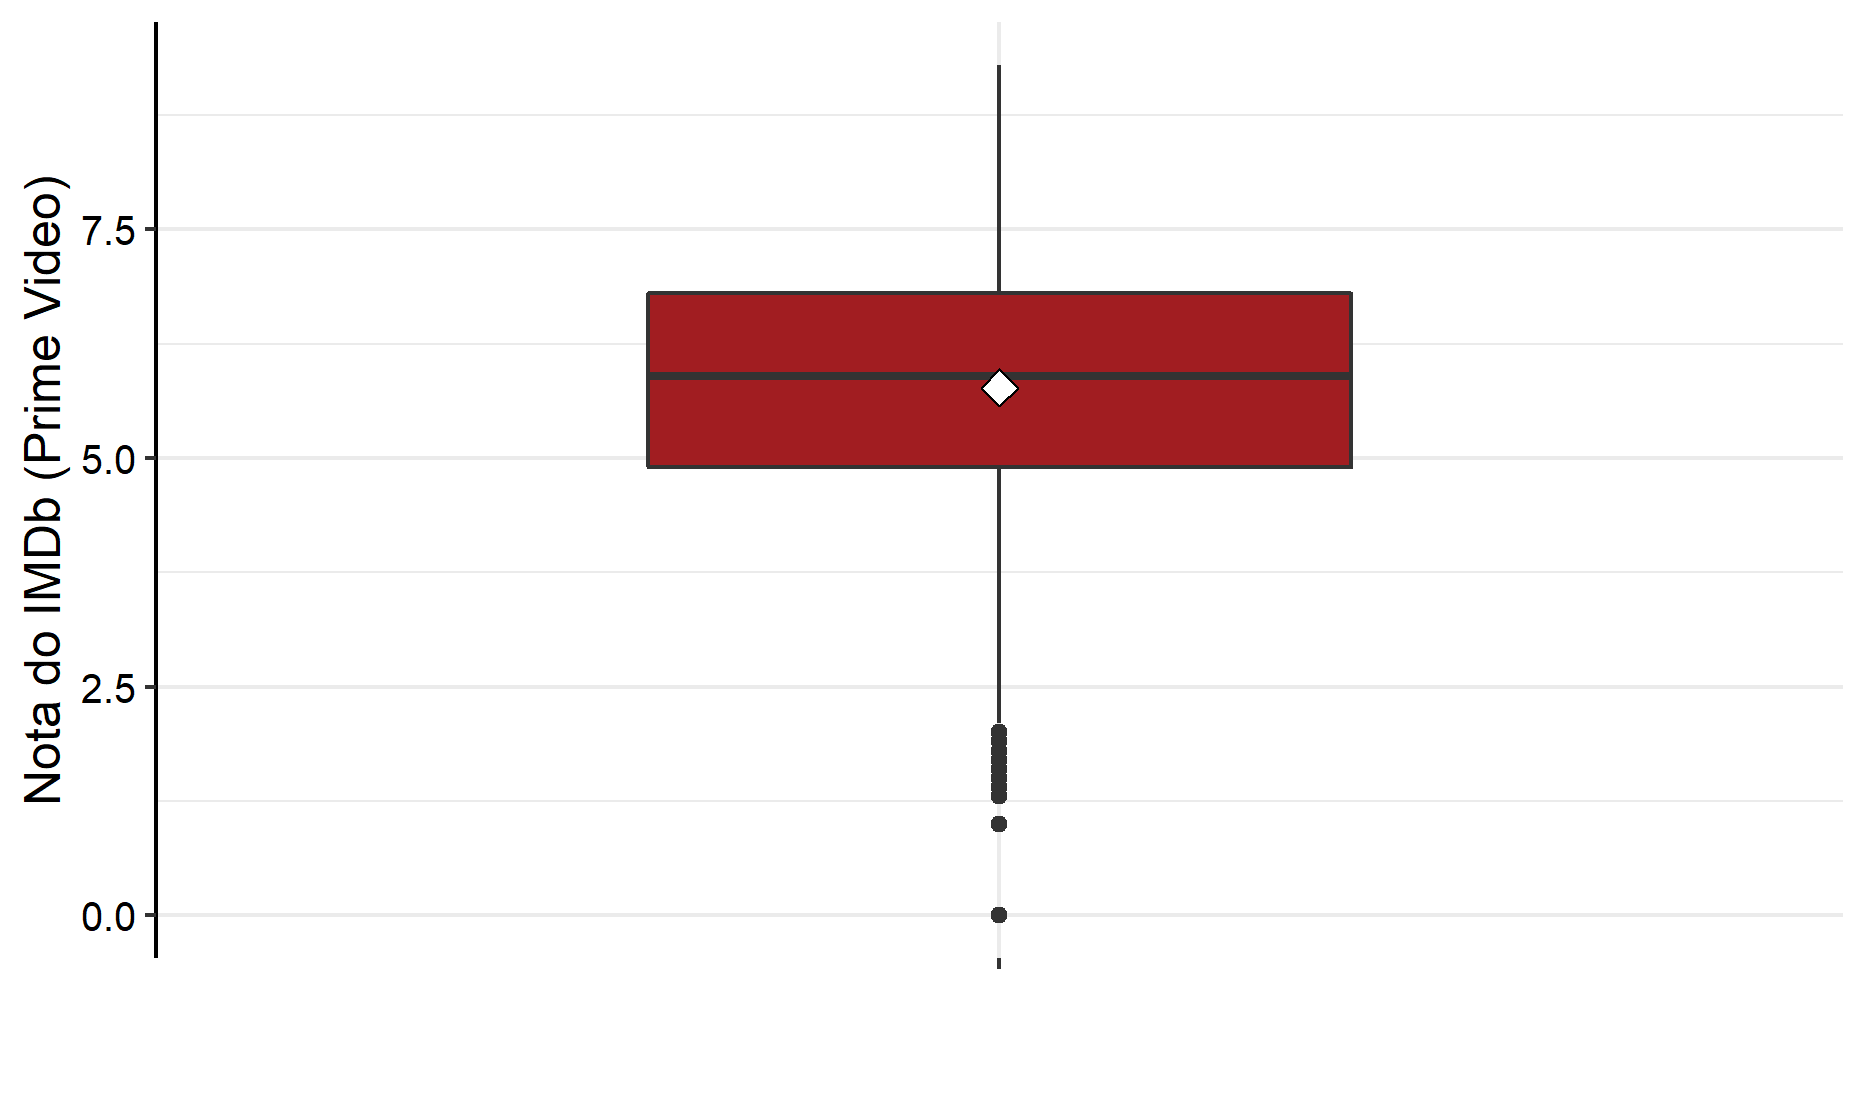
\includegraphics[scale=1]{graf_prime_imdb.png}
\end{figure}

\begin{quadro}[H]
\centering
\label{quadro_resumo1}
\caption{Medidas resumo da variável nota do IMDb}
\begin{tabular}{|c|c|c|} \hline
\textbf{Estatística} & \textbf{Netflix} & \textbf{Prime Video}\\ \hline
Média         & 6,25  & 5,77 \\
Desvio Padrão & 1,139 & 1,397 \\
Mínimo        & 1,4  & 0 \\
1º Quartil    & 5,6  & 4,9 \\
Mediana       & 6,3 & 5,9 \\
3º Quartil    & 7,1 & 6,8 \\
Máximo        & 9,3 & 9,3 \\ \hline
\end{tabular}
\label{quadro_resumo2}
\end{quadro}

Com base nas Figuras 8 e 9 e no Quadro 1, nota-se que as duas plataformas se assemelham significativamente.

Porém, a Netflix supera minimamente o Prime Video, tendo uma média, mediana e quartis mais altos, além de possuir um desvio padrão levemente inferior o que indica notas mais consistentes.

%======================QUESTÃO 6=====================================



\subsection{Top 5 Diretores Segundo a Nota do IMDb}

Esta seção tem como finalidade identificar os 5 diretores com maior média de nota em suas produções. A informação consta no quadro abaixo.

Além disso, o próximo gráfico consta um boxplot das notas médias de todos os diretores, para demonstrar como esta se comporta.

\begin{figure}[H]
\cantering
\caption{Boxplot da variável notas médias dos diretores}
\label{box_uni2}
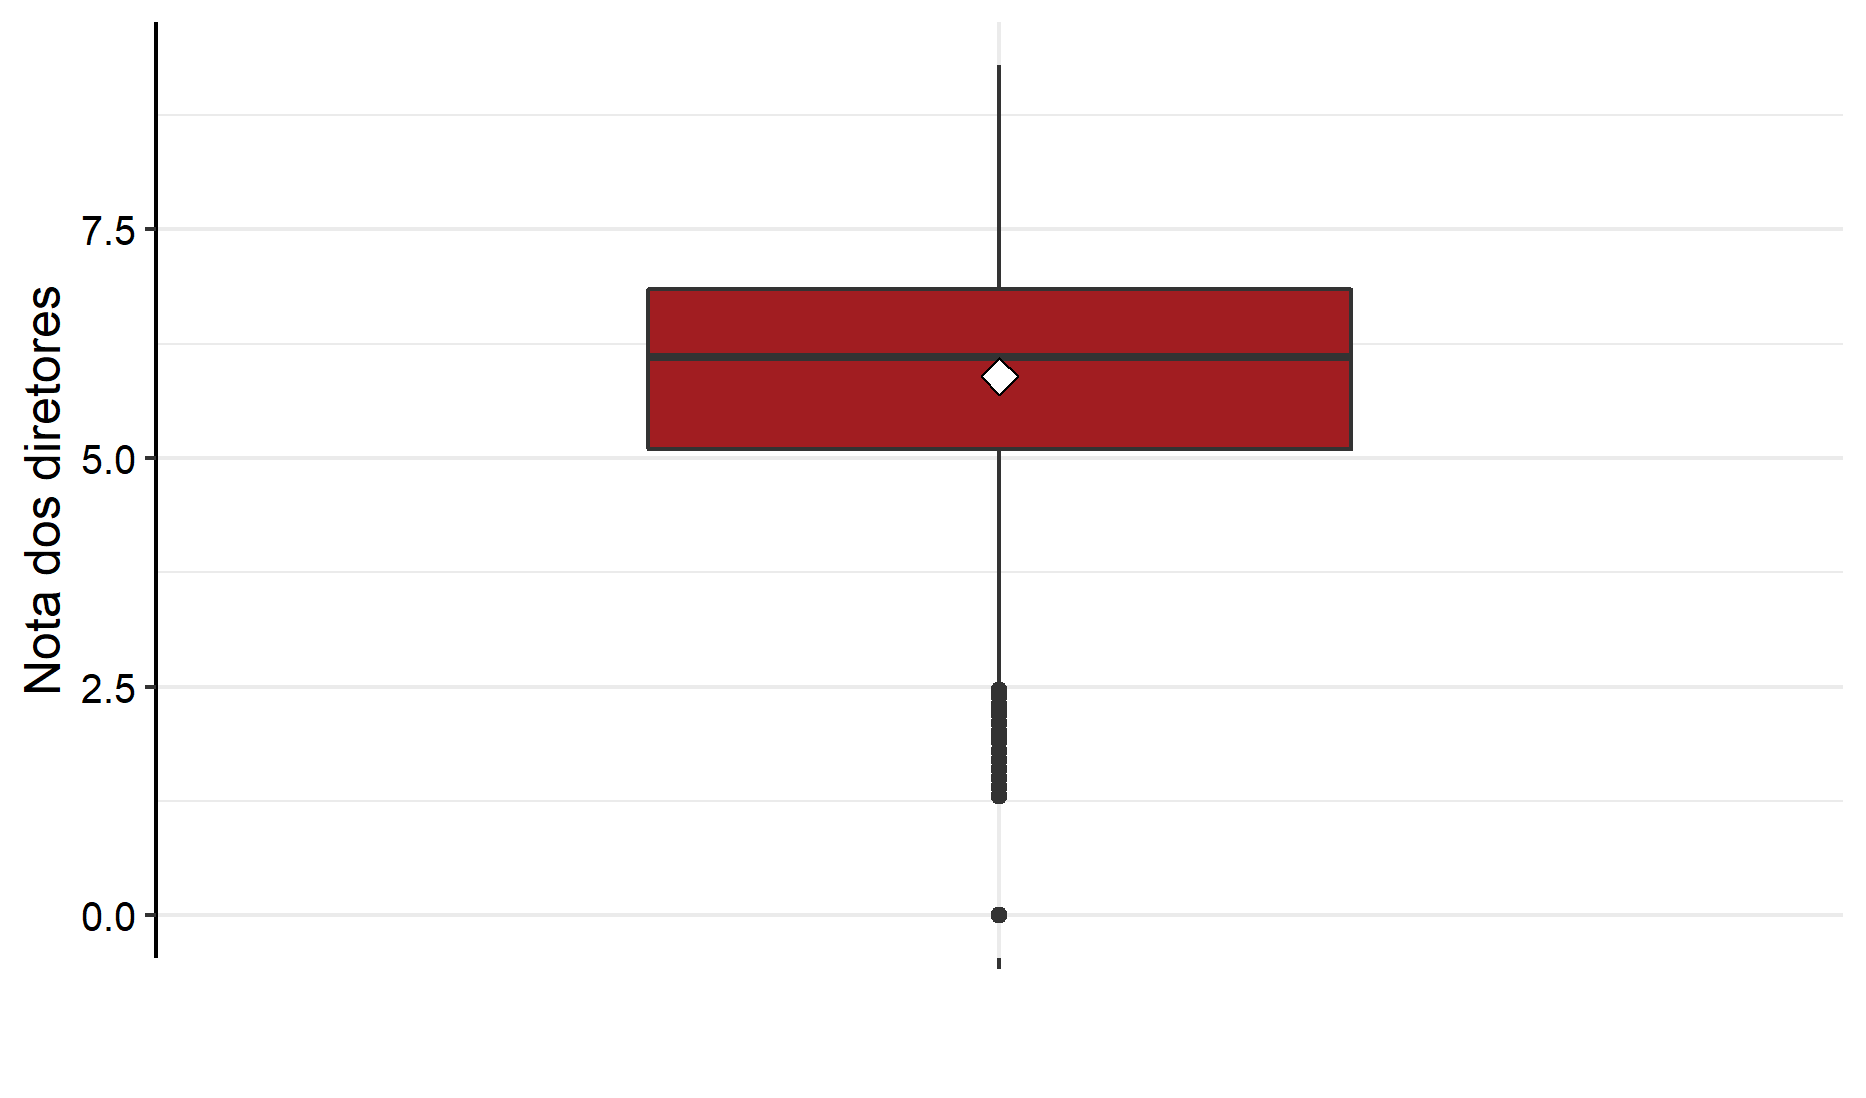
\includegraphics[scale=1]{graf_boxplot_nota_diretores.png}
\end{figure}

\begin{quadro}[H]
\centering
\label{quadro_resumo1}
\caption{Medidas resumo da variável notas médias dos diretores}
\begin{tabular}{|c|c|} \hline
\textbf{Estatística} & \textbf{Notas dos Diretores} \\ \hline
Média         & 5,89   \\
Desvio Padrão & 1,31  \\
Mínimo        & 1.3   \\
1º Quartil    & 5,1   \\
Mediana       & 6,1 \\
3º Quartil    & 6,85  \\
Máximo        & 9,3  \\ \hline
\end{tabular}
\label{quadro_resumo2}
\end{quadro}


\begin{table}[H]
\centering
\caption{Tabela dos melhores 5 diretores}
\begin{tabular}{|c|c|} \hline
\textbf{Diretor} & \textbf{Média de nota no IMDb}\\ \hline
Daany Wu        & 9,3  \\
Fen Tian & 9,3 \\
Miguel Gaudêncio      & 9,3 \\
Chris Leslie, Oggi Tomic    & 9,1 \\
Rel Dowdell       & 9,1 \\ \hline
\end{tabular}
\label{Tabela_1}
\end{table}
%=================================CONCLUSÃO====================
\newpage
\section{Conclusão}

%Portanto, após análise todas as questões sugeridas pelo cliente foram respondidas. 
%Primeiramente, a quantidade de lançamentos de filmes cresce a cada ano, porém em 2020 com o avanço da pandemia de COVID-19 as produções da indústria cinematográfica diminuíram. 
Portanto, não foi detectada relação entre a duração dos filmes e seu ano de lançamento, nem influência da duração dos filmes na nota do Rotten Tomatoes.

A classificação indicativa dos filmes parece se assimilar nas plataformas Netflix, Prime Video e Hulu, enquanto na plataforma Disney a tendência são filmes de classificação indicativa mais baixa (livre ou 7+).

Além disso, as plataformas Prime Video e Netflix tem nota no IMDb bastante similar com uma pequena superioridade da Netflix. Por fim, os melhores diretores estão listados no Quadro 2, lembrando que não foi levada em conta a quantidade de produções do diretor, somente a média da nota de suas produções. 

\end{document}
